\documentclass[12pt,a4paper]{article}
%\renewcommand{\familydefault}{\sfdefault}
\usepackage{amsmath}
\usepackage[a4paper, margin=0.6in]{geometry}
\usepackage{parskip}
\usepackage{tabulary}
\usepackage{float}
\usepackage{titling}
\usepackage{siunitx}
\usepackage{enumitem}

\usepackage[utf8]{inputenc}
\usepackage[english]{babel}
\usepackage{multicol}

\usepackage[]{algorithm2e}

\usepackage{graphicx}

\setlength{\droptitle}{-3em}

\title{COMP4421 Assignment 3}
\author{MOHAMAD, Randitya Setyawan\\20316273\\ \texttt{rsmohamad@ust.hk}}


\begin{document}
	\maketitle
	
	\section*{Exercises}
	\begin{enumerate}
		\item \textbf{Lossless Compression}
			\begin{table}[H]
			\begin{tabular}{|l|l|l|l|l|l|l|l|l|l|l|l|l|}
			\hline
			\multicolumn{3}{|l|}{\textbf{Original Source}}            & \multicolumn{10}{l|}{\textbf{Source Reduction}}                                                                                                                         \\ \hline
			\textbf{Intensity} & \textbf{Prob} & \textbf{Code} & \multicolumn{2}{l|}{\textbf{1}} & \multicolumn{2}{l|}{\textbf{2}} & \multicolumn{2}{l|}{\textbf{3}} & \multicolumn{2}{l|}{\textbf{4}} & \multicolumn{2}{l|}{\textbf{5}} \\ \hline
			1                  & 0.25                 & 10            & 0.25                & 10        & 0.25                 & 10       & \textbf{0.3125}       & 11      & \textbf{0.4375}       & 0       & \textbf{0.5625}       & 1       \\ \hline
			3                  & 0.25                 & 01            & 0.25                & 01        & 0.25                 & 01       & 0.25                  & 10      & 0.3125                & 11      & 0.4375                & 0       \\ \cline{1-9} \cline{11-13} 
			9                  & 0.1875               & 00            & 0.1875              & 00        & 0.1875               & 00       & 0.25                  & 01      & 0.25                  & 10      & \multicolumn{2}{l|}{}           \\ \cline{1-7} \cline{9-13} 
			7                  & 0.125                & 110           & 0.125               & 110       & \textbf{0.1875}      & 111      & 0.1875                & 00      & \multicolumn{4}{l|}{}                                             \\ \cline{1-5} \cline{7-13} 
			2                  & 0.0625               & 1110          & \textbf{0.125}      & 1111      & 0.125                & 110      & \multicolumn{6}{l|}{}                                                                               \\ \cline{1-3} \cline{5-13} 
			12                 & 0.0625               & 11111         & 0.0625              & 1110      & \multicolumn{8}{l|}{}                                                                                                                 \\ \cline{1-1} \cline{3-13} 
			15                 & 0.0625               & 11110         & \multicolumn{10}{l|}{}                                                                                                                                                  \\ \hline
			\end{tabular}
			\end{table}

			\begin{table}[H]
				\begin{tabular}{|l|l|l|l|l|}
				\hline
				\textbf{Intensity} & \textbf{Frequency} & \textbf{Compressed (bits)} & \textbf{Original Size} & \textbf{Compressed Size} \\ \hline
				1                  & 4                  & 2                          & 16                     & 8                        \\ \hline
				3                  & 4                  & 2                          & 16                     & 8                        \\ \hline
				9                  & 3                  & 2                          & 12                     & 6                        \\ \hline
				7                  & 2                  & 3                          & 8                      & 6                        \\ \hline
				2                  & 1                  & 4                          & 4                      & 4                        \\ \hline
				12                 & 1                  & 5                          & 4                      & 5                        \\ \hline
				15                 & 1                  & 5                          & 4                      & 5                        \\ \hline
				\multicolumn{3}{|l|}{\textbf{Total}}                                 & 64                     & 42                       \\ \hline
				\end{tabular}
				\end{table}	

			\begin{align*}
				Compression\ ratio &= uncompressed / compressed &\\
				&= 64/42 \\
				&= 1.5238 
			\end{align*}

		\pagebreak
		\item \textbf{Adaboost Learning Algorithm} \\ \\
		Finding the weights:
		\begin{verbatim}
			T = 1
			Sample weights:
			[0.11111111 0.11111111 0.11111111 0.11111111 0.11111111 0.11111111
			 0.11111111 0.11111111 0.11111111]
			Error = 0.444444
			Classifier weight = 0.111572
			
			T = 2
			Sample weights:
			[0.10557281 0.10557281 0.10557281 0.10557281 0.10557281 0.11803399
			 0.11803399 0.11803399 0.11803399]
			Error = 0.670820
			Classifier weight = -0.355949
			
			T = 3
			Sample weights:
			[0.092548   0.13211548 0.13211548 0.092548   0.092548   0.10347181
			 0.10347181 0.10347181 0.1477096 ]
			Error = 0.288568
			Classifier weight = 0.451175
			
			T = 4
			Sample weights:
			[0.0794725  0.11344975 0.11344975 0.12478422 0.12478422 0.139513
			 0.08885295 0.08885295 0.12684067]
			Error = 0.750432
			Classifier weight = -0.550458
			
			T = 5
			Sample weights:
			[0.06716772 0.09588425 0.09588425 0.18287912 0.18287912 0.11791211
			 0.07509579 0.07509579 0.10720185]
			Error = 0.538358
			Classifier weight = -0.076866

		
		\end{verbatim}

		\begin{enumerate}
			\item H3 and H1 have the highest weights. Final classifier:
			\begin{flalign*}
				H(\textbf{x}) &= sgn(0.4512 \cdot h_3(\textbf{x}) + 0.1116 \cdot h_1(\textbf{x}))
			\end{flalign*}

			\item Final classifier response:
			\begin{verbatim}
				[1, 1, -1, 1, -1, -1, -1, 1, -1]
			\end{verbatim}
		\end{enumerate}
	\end{enumerate}

	\pagebreak
	\section*{Programming}
	\begin{enumerate}
		\item \textbf{Digit Segmentation} \\
		I used the given segmentation algoritm (row and column projections) with additional preprocessing and different method to handle digits that are close. \\

		\begin{itemize}
			\item \textbf{Step 1}: Clean and binarize the image
			\begin{itemize}
				\item Convert the image to grayscale
				\item Obtain the background (image sans digits) by dilating the grayscale image
				\item Subtract the background to get a clean image of digits
				\item Binarize the digits using OTSU algorithm
			\end{itemize}
			\item \textbf{Step 2}: Separate the rows using the y-projections on the binarized image
			\item \textbf{Step 3}: Separate the columns in each row using x-projections
			\item \textbf{Step 4}: Create ROIs using the obtained rows and columns
			\item \textbf{Step 5}: Each ROI may contain 2 close digits, separate them by finding connected components
		\end{itemize}

		\textbf{1.jpg} \\
		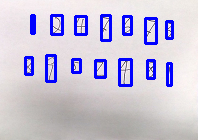
\includegraphics[width=0.6\textwidth]{./result_images/digits_of_image_1/1_segmented.png}

		\pagebreak
		\textbf{2.bmp} \\
		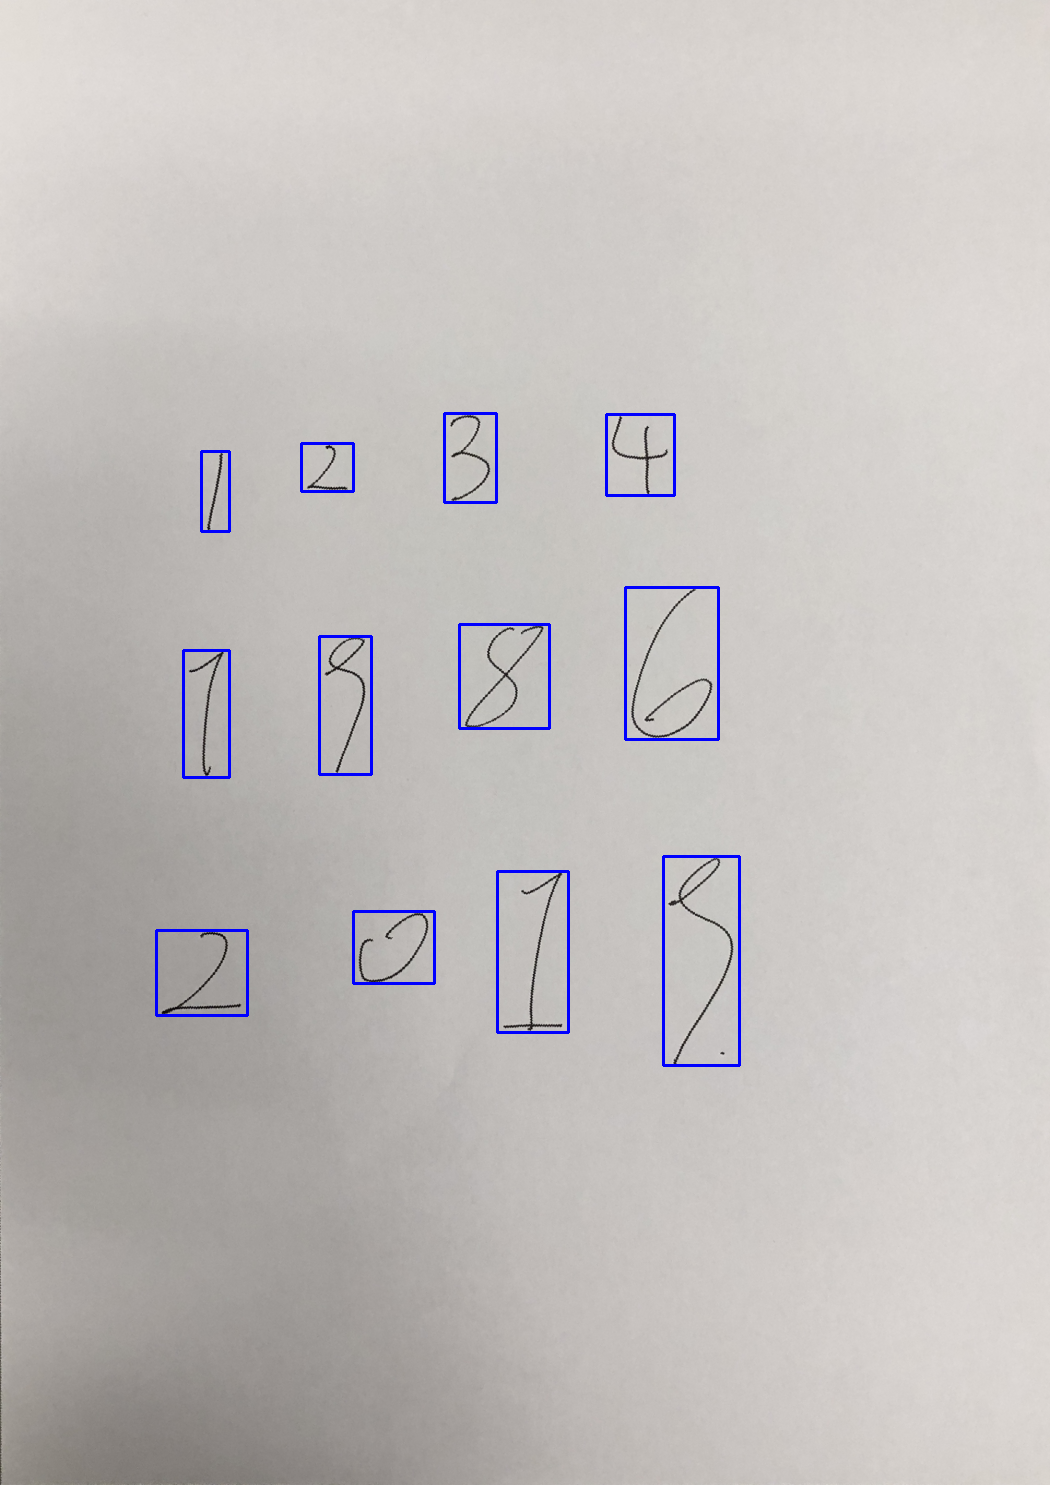
\includegraphics[width=0.6\textwidth]{./result_images/digits_of_image_2/2_segmented.png}

		\textbf{3.bmp} \\
		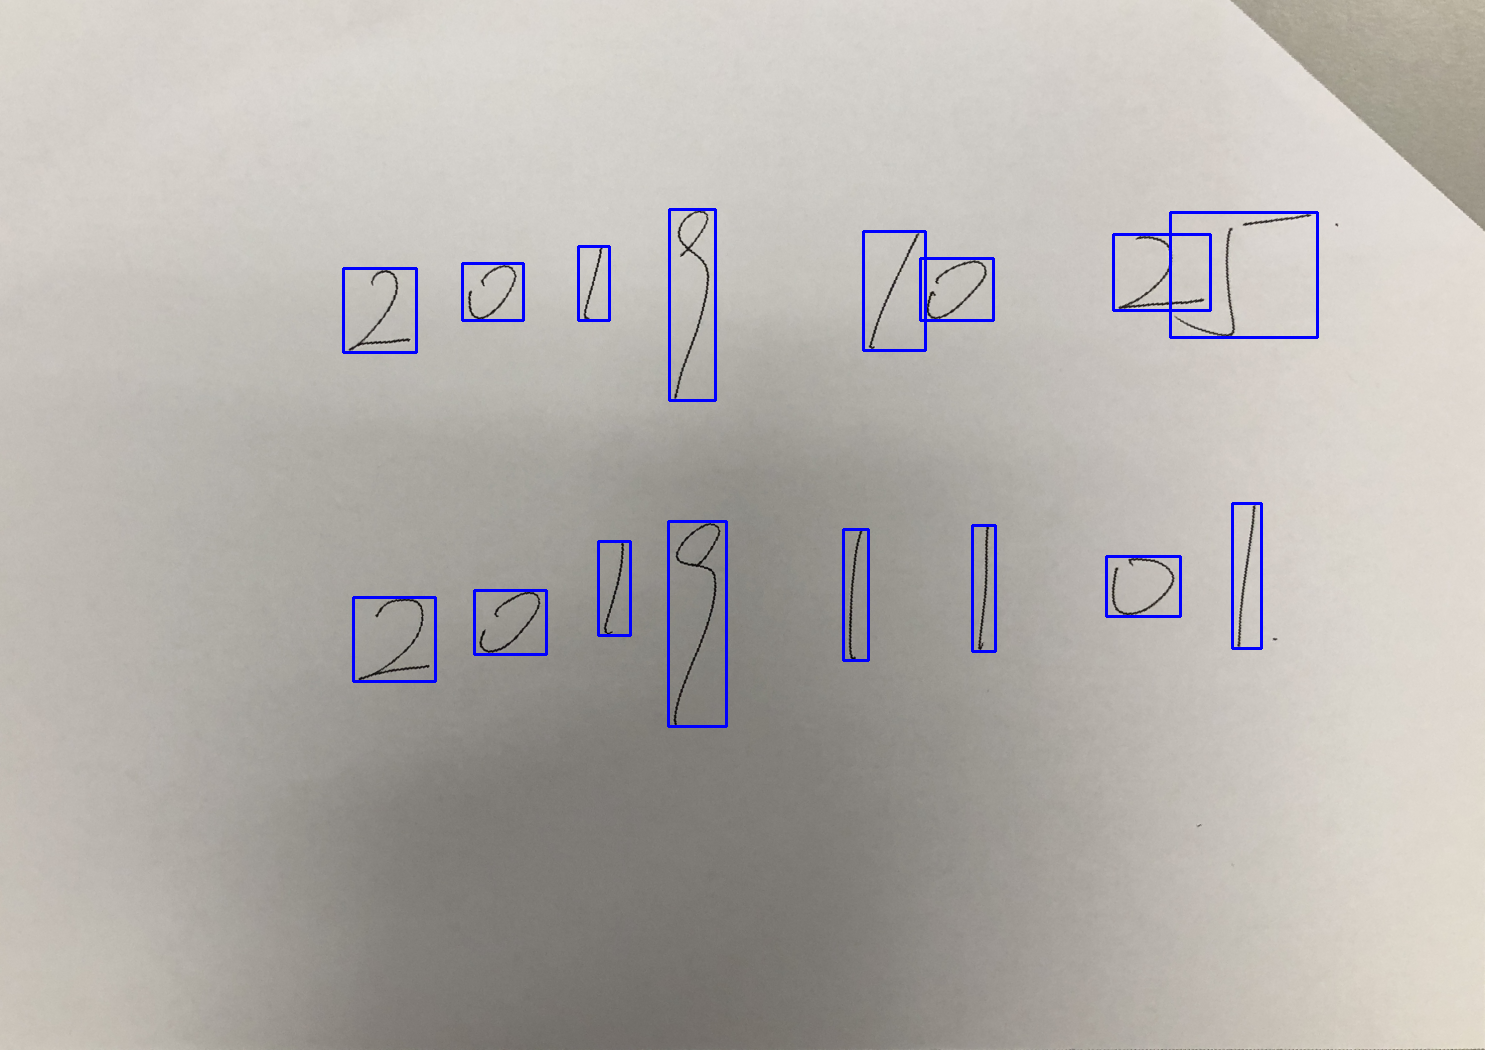
\includegraphics[width=0.6\textwidth]{./result_images/digits_of_image_3/3_segmented.png}


		\pagebreak
		\item \textbf{Adaboost Classification} \\
		I used 5 decision trees for the weak classifiers

		\textbf{1.jpg} - accuracy=0.6429\\
		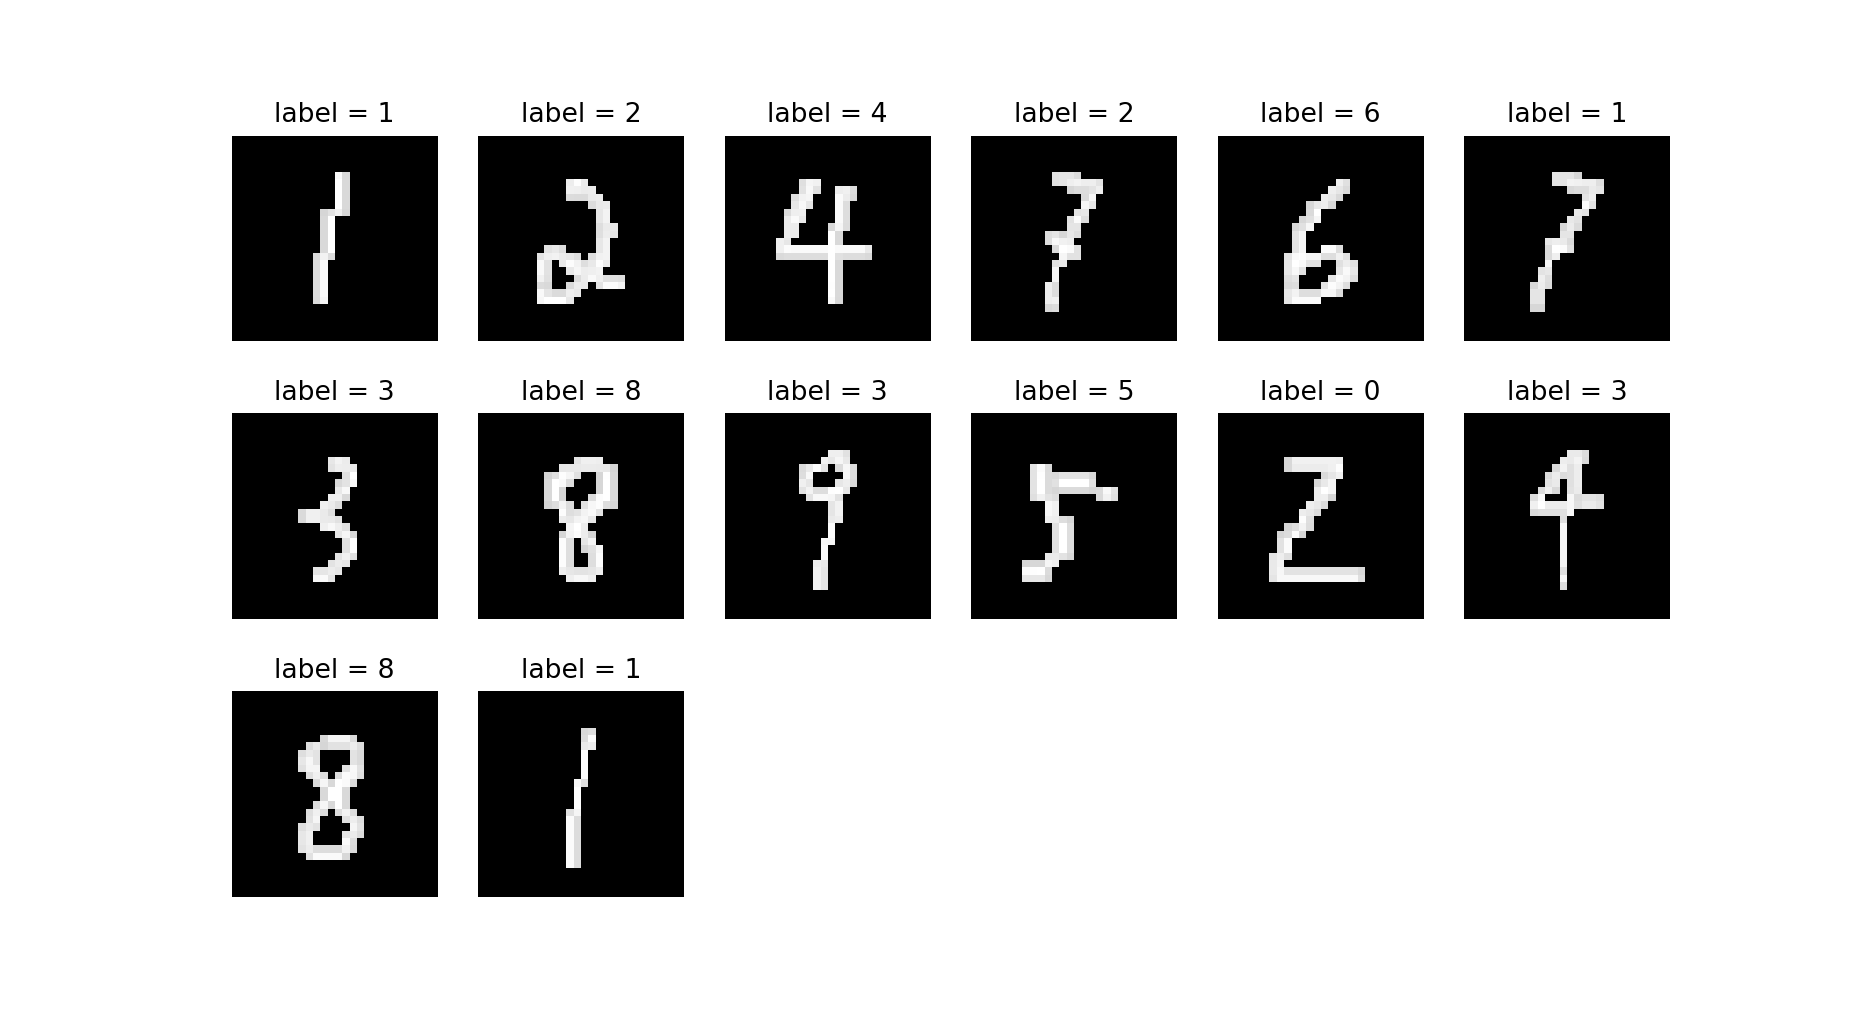
\includegraphics[width=0.9\textwidth]{./result_images/digits_of_image_1/1_label.png}

		\textbf{2.bmp} - accuracy=0.833 \\
		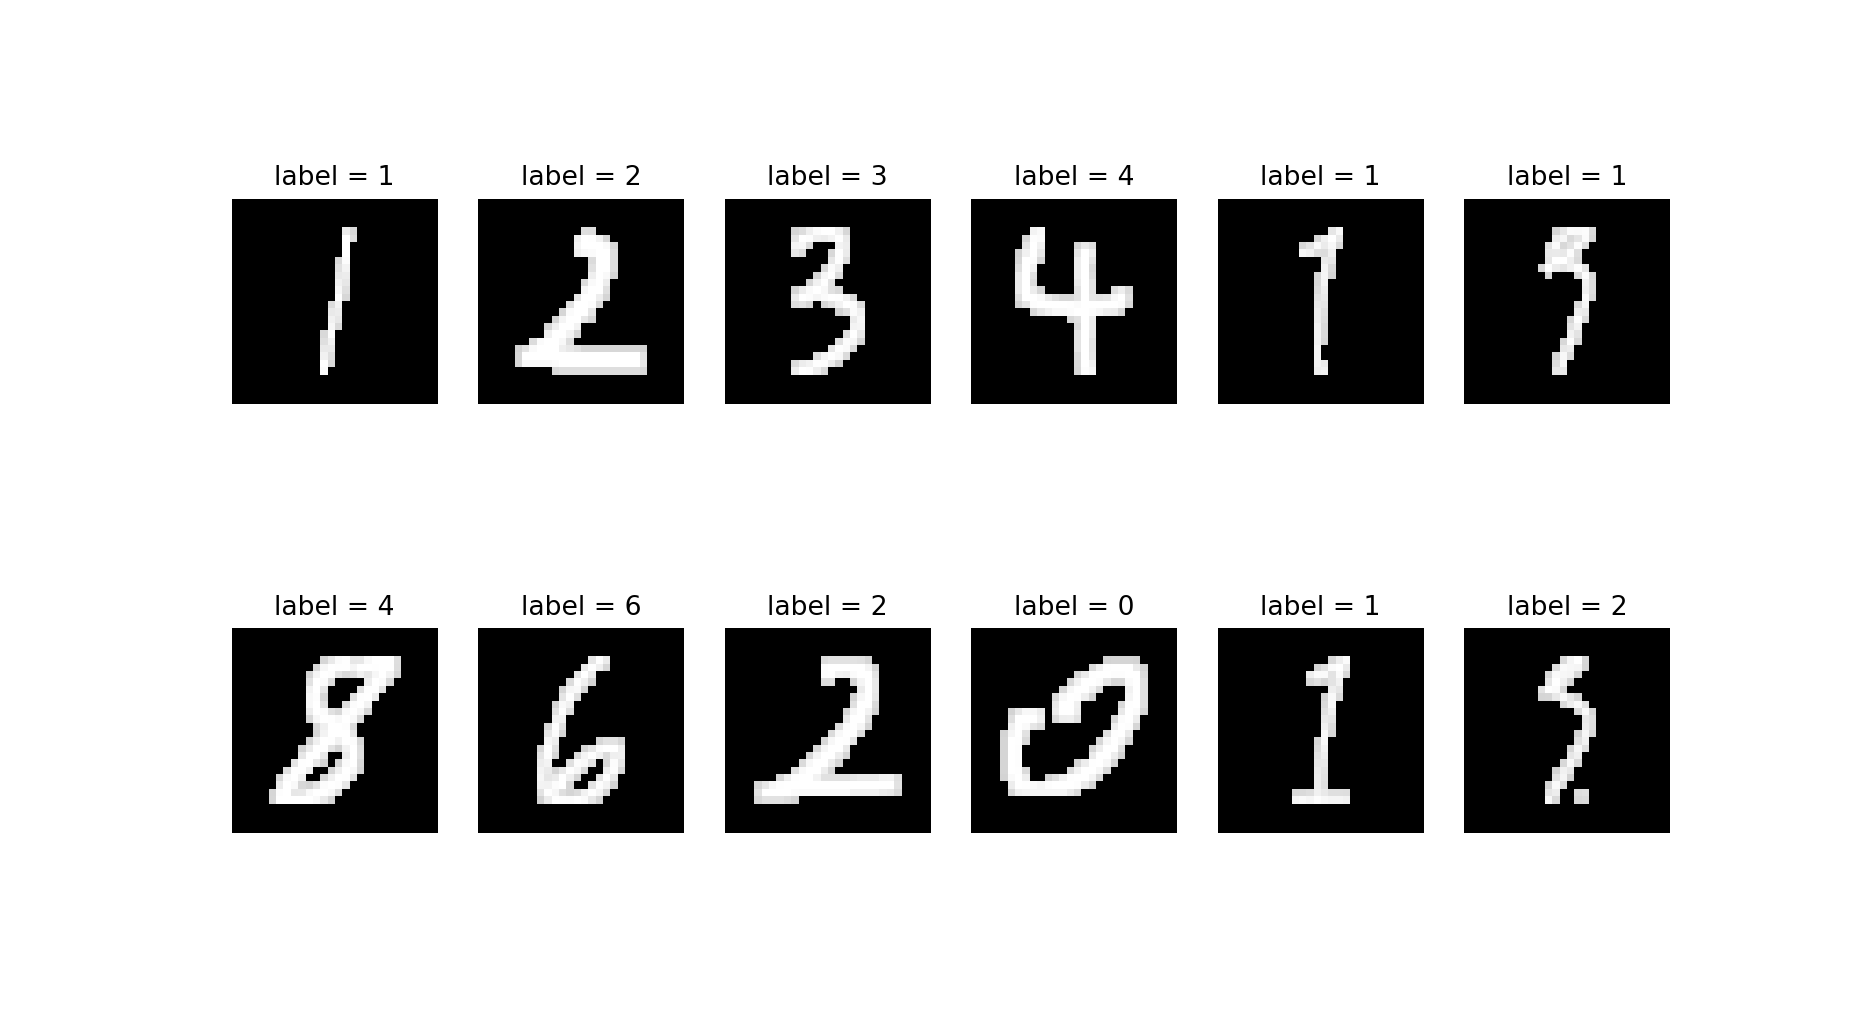
\includegraphics[width=0.9\textwidth]{./result_images/digits_of_image_2/2_label.png}

		\pagebreak
		\textbf{3.bmp} - accuracy=0.8125 \\
		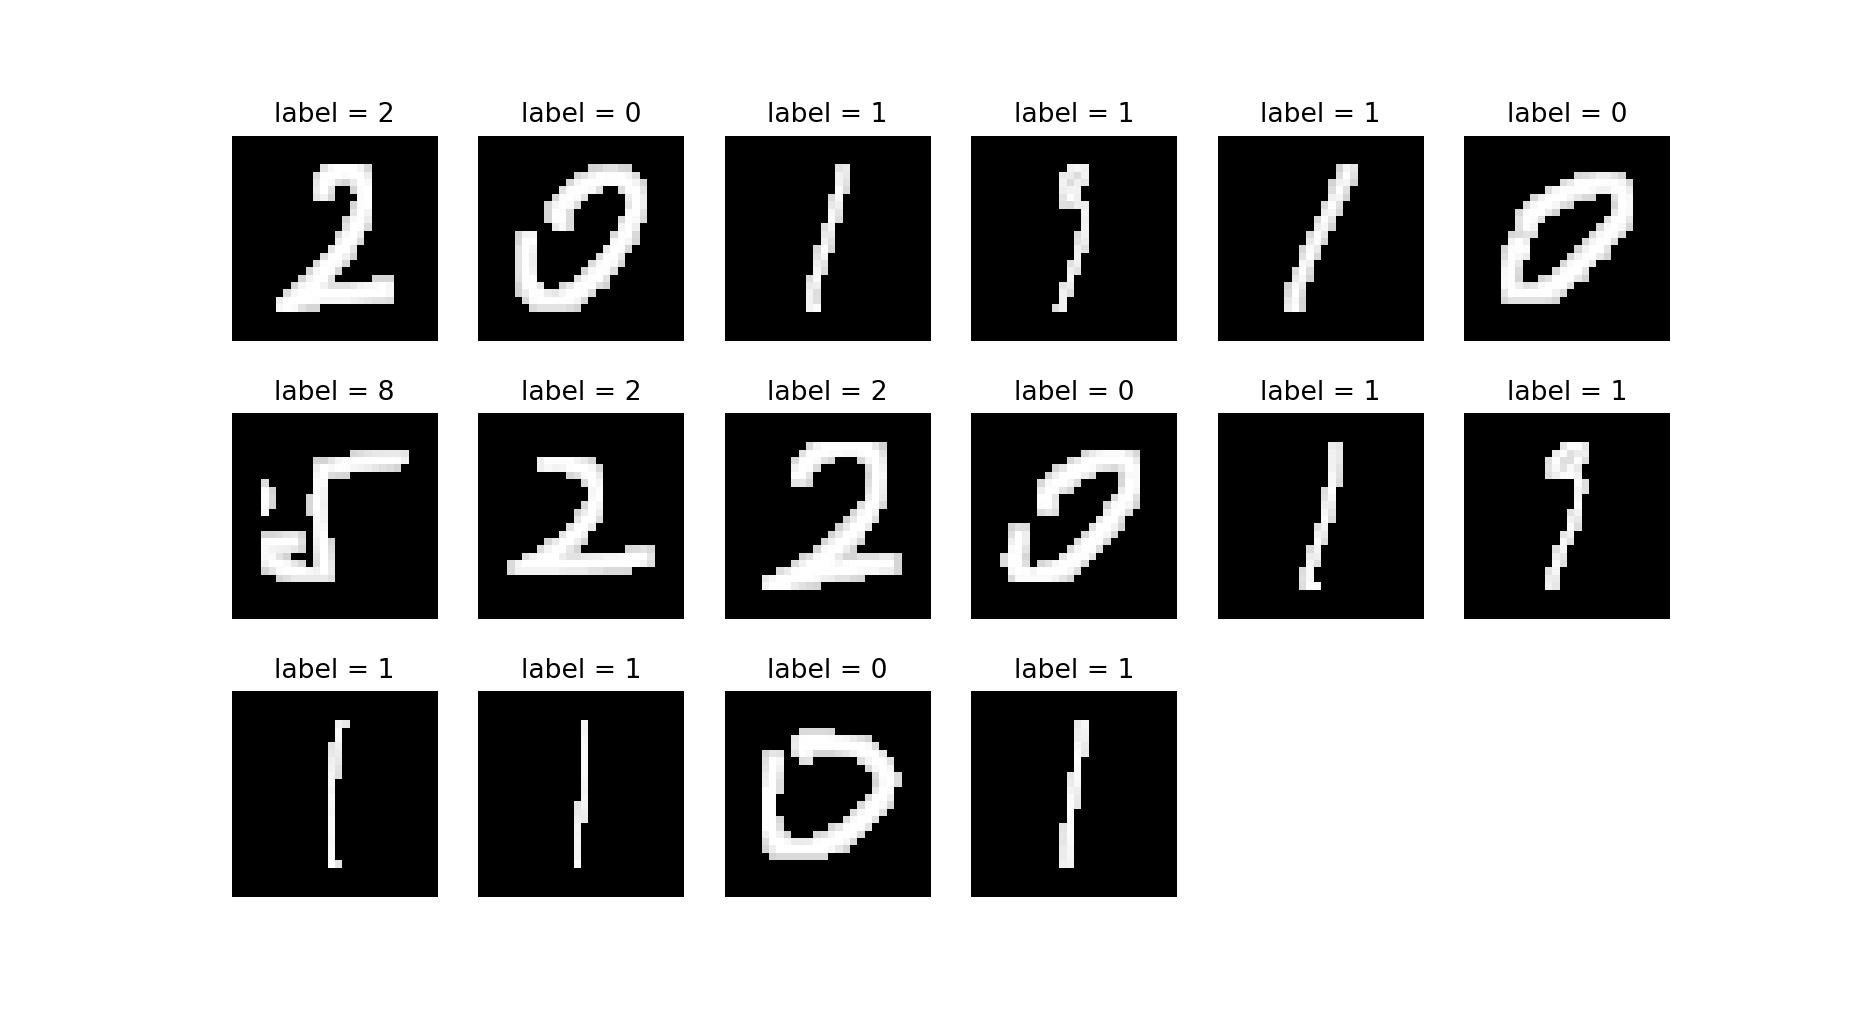
\includegraphics[width=0.9\textwidth]{./result_images/digits_of_image_3/3_label.png}



	\end{enumerate}
		
\end{document}

